\documentclass[12pt, a4paper]{article}

\usepackage{graphicx}
\usepackage{float}
\usepackage{hyperref}
\usepackage{siunitx}
\usepackage{amsmath}

\begin{document}
	\pagenumbering{gobble}
		\begin{titlepage}
			\centering
			{\LARGE Controls Systems Practical 4 \par}
			\vspace*{1.5cm}
			{\large Q. Kruger, 216008466 \par}
			{\large R. de Bruyn, 216054484 \par}
			\vspace*{1.2cm}
			{\large \today}
			\vspace*{\fill}
			% 
\includegraphics[width=\textwidth]{img/UJ.jpg}
			\vspace*{\fill}
		\end{titlepage}

		\pagenumbering{roman}
		\tableofcontents
		\listoffigures
		\newpage
		\pagenumbering{arabic}

		\section{Pre Lab} % (fold)
		\label{sec:pre_lab}

		\subsection{Question 1} % (fold)
		\label{ssub:question_1}
		Considering 3 cascaded blocks each with a transfer function given as $G_1 = \frac{1}{s+1}$, $G_2 = \frac{1}{s+4}$ and $G_3 = \frac{s+3}{s+5}$ respectively. The equivalent transfer function of this system is given below

		\begin{equation}
			\begin{array}{rcl}
				G & = & G_1 \times G_2 \times G_3\\
				  & = & \frac{1}{s+1} \times \frac{s}{s+4} \times \frac{s+3}{s+5}\\
				  & = & \frac{s+3}{s^3+10s^2+29s+20}
			\end{array}
		\end{equation}
		
		% subsubsection question_1 (end)

		\subsection{Question 2} % (fold)
		\label{sub:question_2}
		The equivalent transfer function of 3 blocks in parallel with transfer functions given as $G_1 = \frac{1}{s+1}$,$G_2 = \frac{1}{s+4}$ and $G_3 = \frac{s+3}{s+5}$ respectively is given below

		\begin{equation}
			\begin{array}{rcl}
				G & = & G_1 + G_2 + G_3\\
				  & = & \frac{(s+4)(s+5)+(s+1)(s+5)+(s+3)(s+1)(s+4)}{(s+1)(s+4)(s+5)}\\
				  & = & \frac{s^2+9s+9+s^2+6s+5+s^3+4s^2+16s+3s+12}{s^3+5s^2+4s+5s^2+25s+20}\\
				  & = & \frac{6s^2+34s+21}{s^3+10s^2+29s+20}
			\end{array}
		\end{equation}		
		% subsection question_2 (end)

		\subsection{Question 3} % (fold)
		\label{sub:question_3}
			\[
				\begin{array}{rcl}
					T(S) & = & \frac{G(s)}{1 + G(s)H(s)} \\
					& = & \frac{s+1}{s(s+2)} \,\div\, \left(1 + \frac{(s+1)(s+3)}{s(s+2)(s+4)} \right) \\
					& = & \frac{s+1}{s(s+2)} \,\cdot\, \left(\frac{s(s+2)(s+4)}{s(s^2 + 4s + 8) + s^2 + 4s + 3} \right) \\
					& = & \frac{s^2 + 5s + 4}{s^3 + 7s^2 + 12s + 3}
				\end{array}
			\]
		% subsection question_3 (end)

		\subsection{Question 4} % (fold)
		\label{sub:question_4}
			\[
				T(s) = \frac{G(s)H(s)}{1 + G(s)}
			\]
		% subsection question_4 (end)

		\subsection{Question 5} % (fold)
		\label{sub:question_5}
			\[
				T(s) = \frac{G(s)H(s)}{1 + G(s)}
			\]
		% subsection question_5 (end)
		
		% section pre_lab (end)

		\section{Lab} % (fold)
		\label{sec:lab}

		\subsection{Question 1} % (fold)
		\label{sub:question_1}
		By giving the transfer functions $G_1$, $G_2$, $G_3$ and $G$ as given in the prelab section of this report Question 1 and running the \texttt{step} functions on the respective transfer functions in Octave, the following plots were obtained as shown in Figure \ref{fig:question_1_lab} 

		\begin{figure}[H]
			\centering
			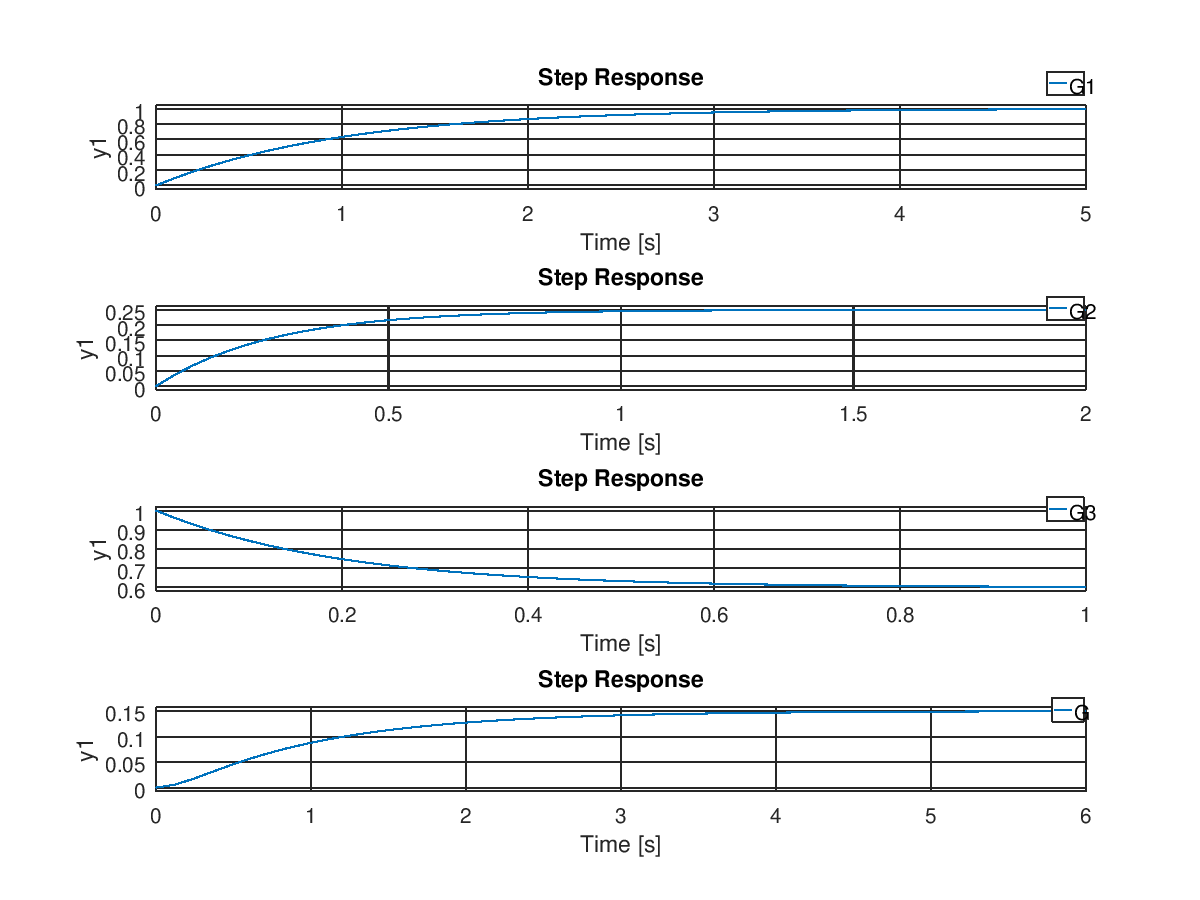
\includegraphics[width=0.7\textwidth]{Images/question_1_lab.png}
			\caption{Step function of the respective transfer functions as in Question 1 of the prelab}
			\label{fig:question_1_lab} 
		\end{figure}
		
		By using MATLAB's \texttt{stepinfo} function on these transfer functions respectively we were able to obtain the  settling time and rise time for each transfer function. \\
		.\\
		.\\
		.\\
		.\\
		.\\
		.\\
		% subsection question_1 (end)

		\subsection{Question 2} % (fold)
		\label{sub:question_2}
		By running the \texttt{step} function on the transfer function of Question 2 in the prelab the individual plots are shown by \ref{fig:question_2_lab}

		\begin{figure}[H]
			\centering
			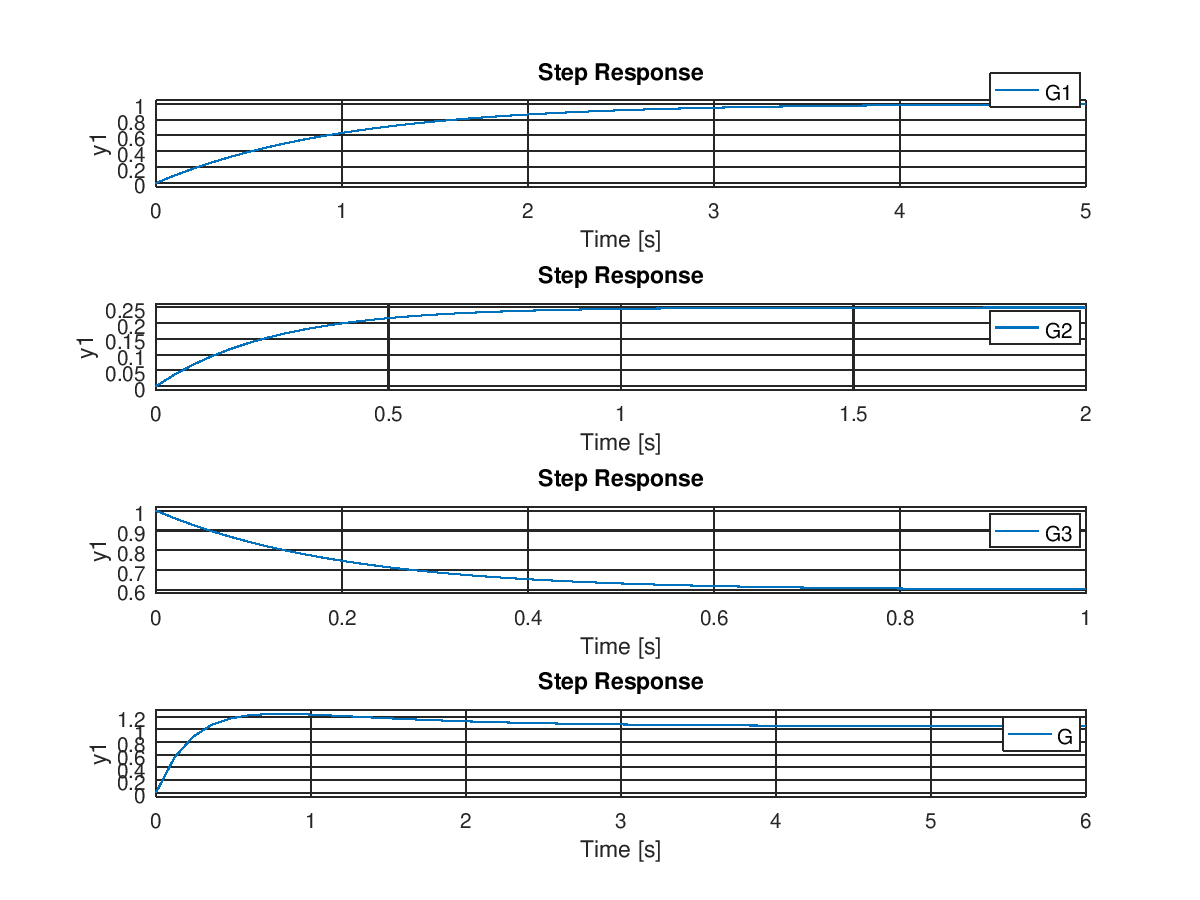
\includegraphics[width=0.7\textwidth]{Images/question_2_lab.png}
			\caption{Step function of the respective transfer functions as in Question 2 of the prelab}
			\label{fig:question_2_lab} 
		\end{figure}

		By using MATLAB's \texttt{stepinfo} function on these transfer functions respectively we were able to obtain the  settling time and rise time for each transfer function. \\
		.\\
		.\\
		.\\
		.\\
		.\\
		.\\

		
		% subsection question_2 (end)

		\subsection{Question 4} % (fold)
		\label{sub:question_4}
			Figures \ref{fig:4_1} and \ref{fig:4_2} show the step response plots of the transfer functions given in prelabs 3, 4, and 5. Note that prelabs 4 and 5 have the same transfer function, so figure \ref{fig:4_2}	represents both transfer functions.
			\begin{figure}[H]
				\centering
				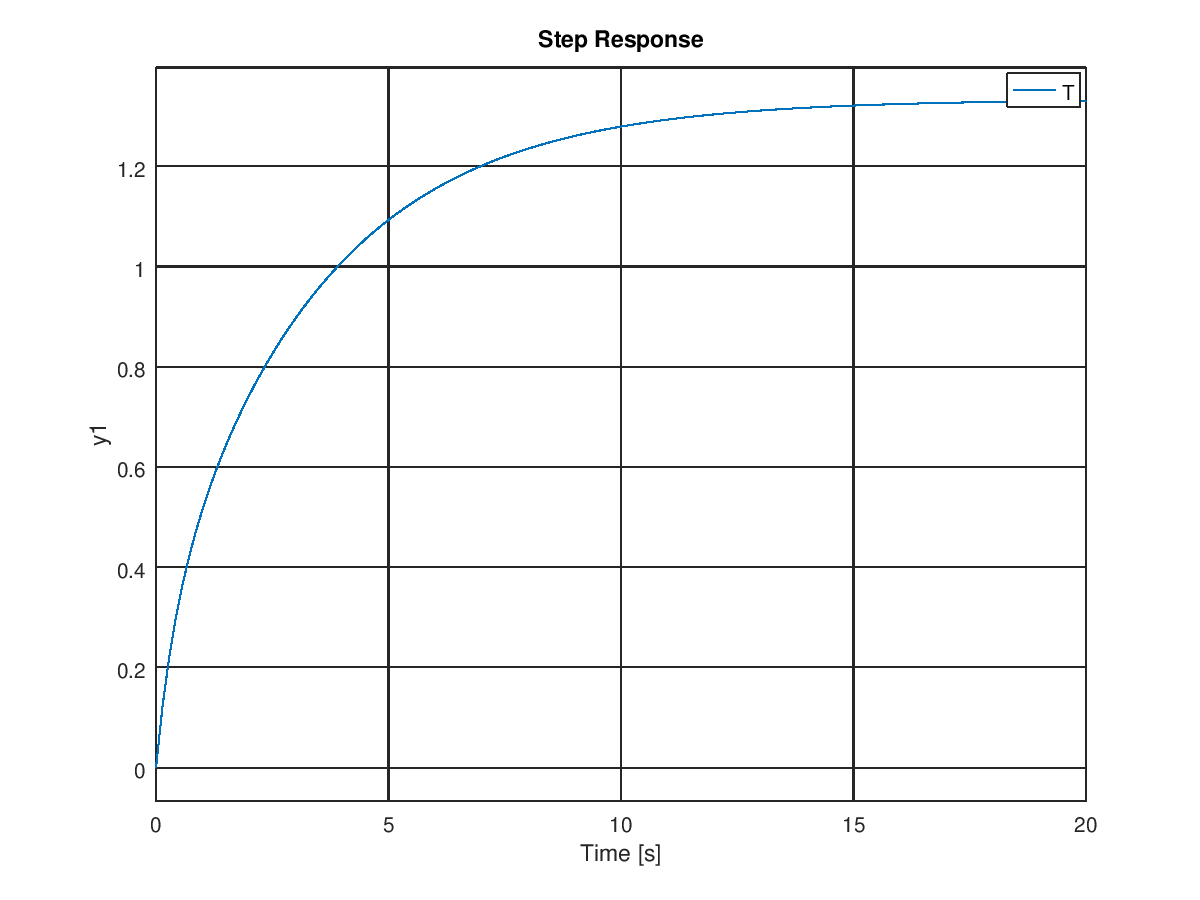
\includegraphics[width=0.7\textwidth]{Images/question_4_1_lab.png}
				\caption{Step function of prelab question 3}
				\label{fig:4_1} 
			\end{figure}

			\begin{figure}[H]
				\centering
				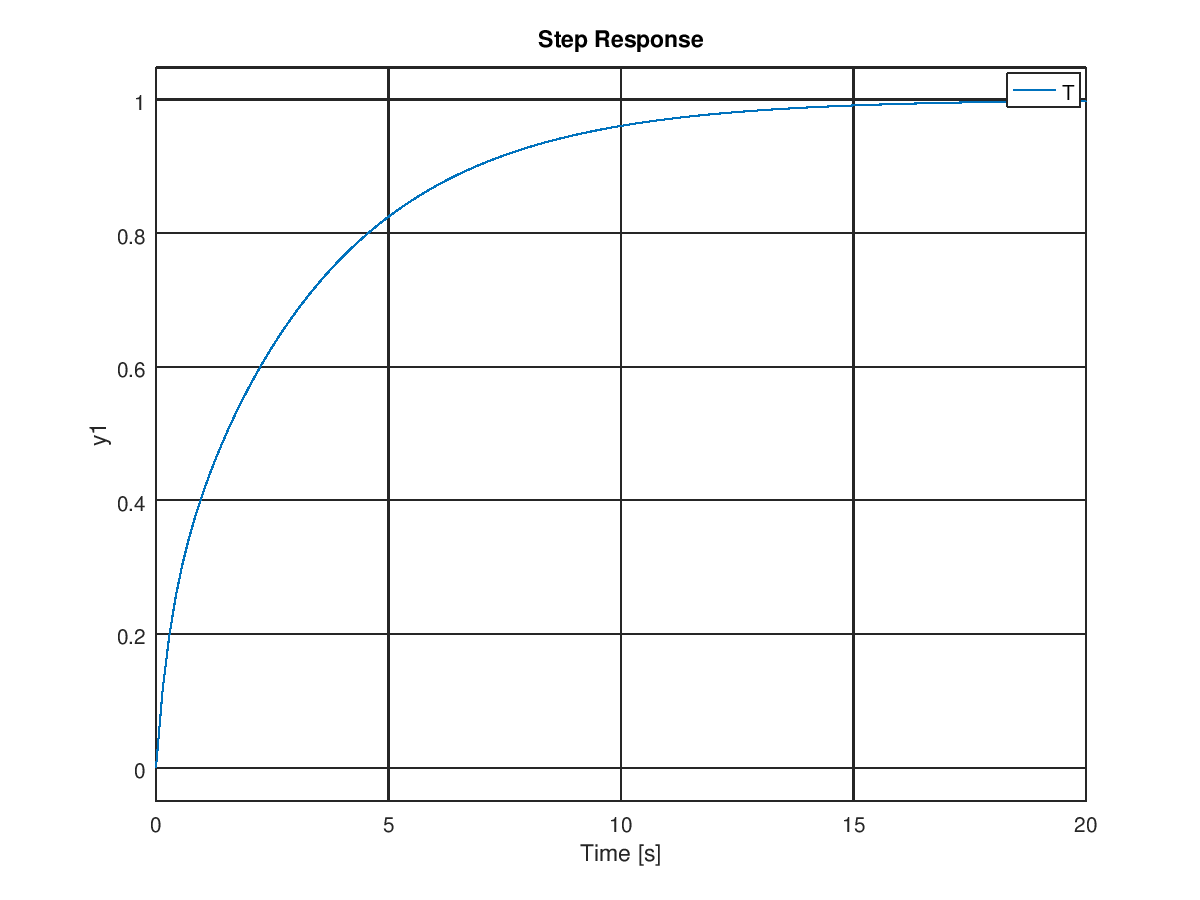
\includegraphics[width=0.7\textwidth]{Images/question_4_2_lab.png}
				\caption{Step function of prelab question 4 and 5}
				\label{fig:4_2} 
			\end{figure}
		% subsection question_4 (end)
		
		% section lab (end)

\end{document}